\documentclass{article}
\usepackage{fixltx2e}
\usepackage{float}
\usepackage{amsmath}
\newcommand{\degree}{\ensuremath{^\circ}}
\usepackage{graphicx}
\usepackage[margin=1.0in]{geometry}
\usepackage{subfigure}
\usepackage{caption}
\linespread{1.5}


\title{Overfishing: An Agent-Based Model in Matlab}
		
\author{Michael Lee \\ The University of Texas at Austin}

\begin{document}
\maketitle{}

The model uses an agent-based approach to simulate the effects of overfishing on the distribution of both the fish and fishermen. After an initial distribution of fish stocks is generated, each agent choses to relocate to the best location in his proximity based upon the available reserves of fish. The stock of fish at each location is dynamic, depleting and regenerating as a function of the level of resource recovery experienced. The final result is the spatial distribution of agents as a function of the spatial distribution of the fish. Since 

\newpage

\section{Base Model}
The original model found in Computational Economics (Kendrick et. al, 2006), derived from the work of Joshua M. Epstein and Robert Axtell (1996), develops a two-peak sugarscape model, i.e. a spatial distribution having two high-resource regions. Agents are randomly created, each having two fixed and two dynamic qualities: vision, metabolism, state, and wealth. Vision refers to the number of nodes away the agent can "see" or evaluate, metabolism how many resources are consumed from the node each period, state whether the agent is active or not, and wealth the total number of resources consumed over time. The sugarscape distribution is generated once and has a resource recovery rate \emph{$G_{\inf}$}, meaning that the distribution regenerates completely thus remaining static. \*

Agents are selected in a random order to evaluate their surroundings and, if necessary, move to a better, unoccupied location. This procedure is carried out for a predetermined number of runs, with the spatial distribution of the agents plotted each time. Since \emph{$G_{\inf}$}, as the number of time periods reaches infinity, the agents will form clusters identical to the sugar peaks.   \*

\section{Overfishing}
I wanted to apply this style of agent-based computation economics (ACE) to the problem of overfishing. Since the 1950's, large-scale industrial fishing has led to a dramatic fall in fish population, under 10\% of their pre-industrial levels by some estimates (National Geographic).

\begin{figure}[!ht]
\begin{center}
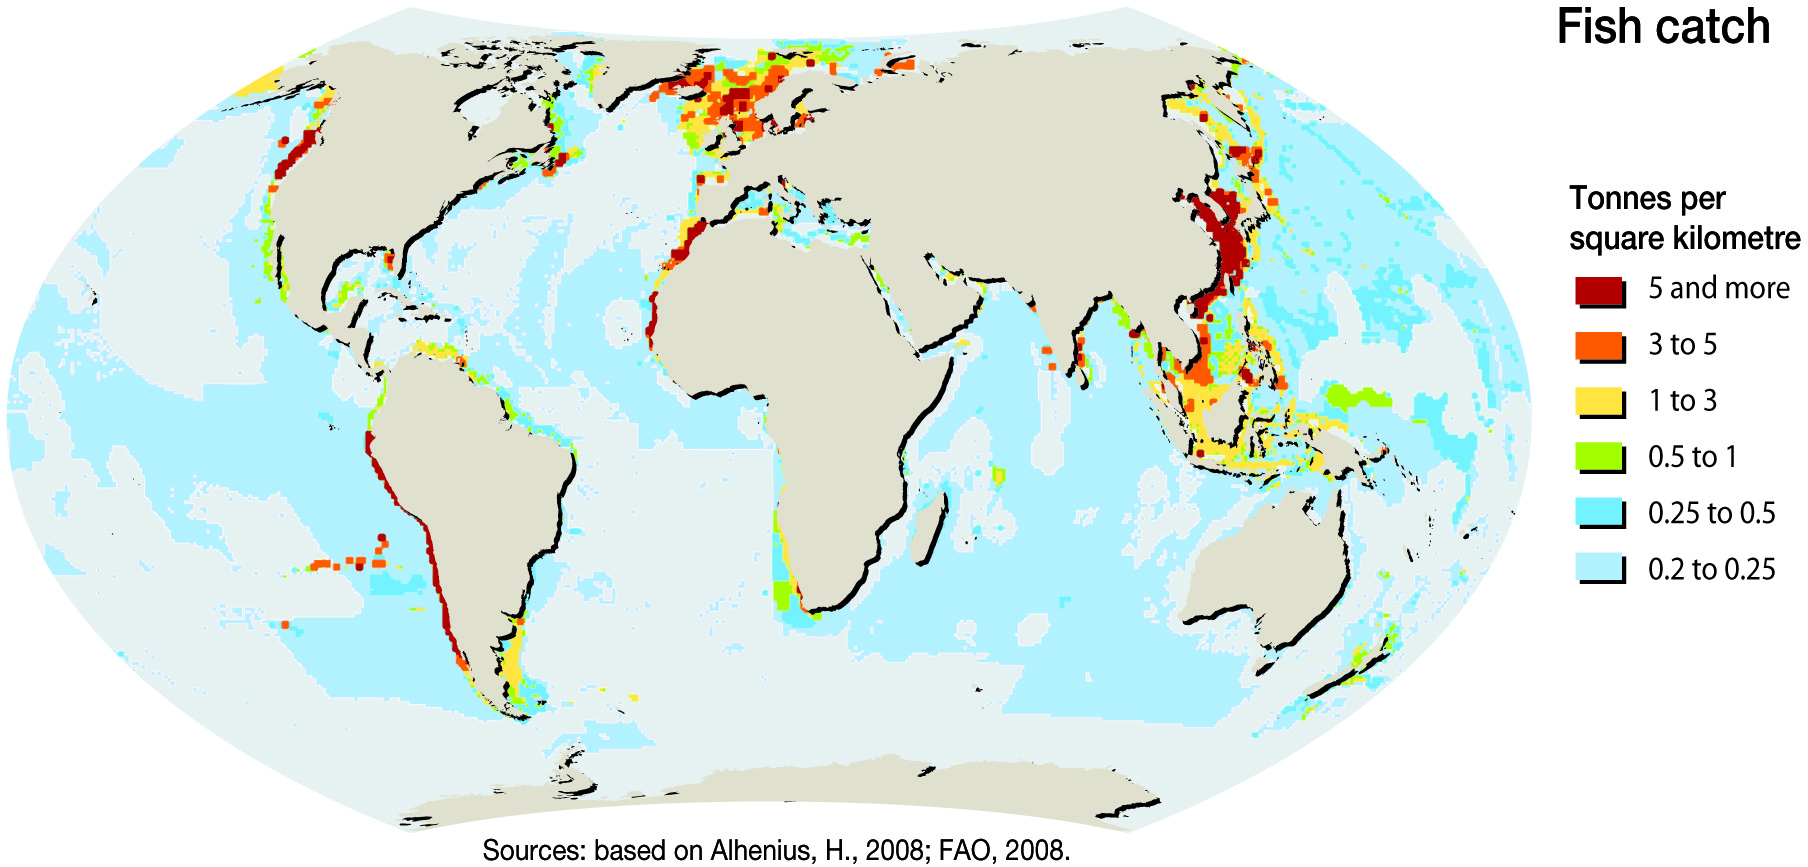
\includegraphics[scale=.25]{fish.jpg}
\caption{The World's Fish Catch 2008}
\end{center}
\end{figure}

The problem is compounded as developing countries become more protein hungry, and look to the oceans for a source of cheap, lean protein. This strain on the local fish supply causes the overall supply of fish to fall, as the fish most sought after commercially-- large ones-- disproportionally account for the species reproduction. This has causes traditional fishing hotspots to become "dead zones" or regions where no fish inhabit\*

\section{An Agent-Based Overfishing Model}
The model aims to show how the spatial distribution of fishermen distorts the natural ecology by depleting the fish supply. As agent \emph{$A_{i}$} with metabolism \emph{$M_{i}$} moves into a node, it consumes the magnitude of \emph{$M_{i}$} from the available fish supply of the node. \*

The fundamental difference between this model and the base model is that the resource supply is not fully replenished after each run and instead is regenerated or depleted based on the level of fishing at each node. However, it is not just the level of fishing at each individual node, but the level at all surrounding nodes as well. Let $\delta$ denote the global depletion rate and $\rho$ the global regeneration rate. If the node is being fished on:

\begin{equation}
	Depletion_{i,j} = - \frac{[M_{i,j} + M_{i+1, j} + M_{i-1, j} + M_{i, j+1} + M_{i, j-1}]}{\delta} + 1
\end{equation}

{\bf Equation 1} is the equivalent to the two-dimensional convolution matrix, a type of Fourier Transform used frequently in signal and image processing, which is a concise way of finding the sum of all adjacent elements. \\
If the node is not being fished on, then the stock is regenerated as described by {\bf Equation 2}: 

\begin{equation}
	Regeneration_{i,j} = \frac{\rho}{[M_{i+1, j} + M_{i-1, j} + M_{i, j+1} + M_{i, j-1}]} + 1
\end{equation}

Both {\bf equation 1} and {\bf 2} are created in the belief that if many people are fishing in the areas next you, the fish in your area are less likely to reproduce thus depleting the stock. By the formulation in {\bf equation 2}, even if no one is fishing on a node, if its surroundings are heavily fished then its stocks will be depleted as well. \*

Similar to the base model, each agent will choose to go to a new location based on the amount of available resources, however, in this model the agent's decision is also determined by the number of people interacting with the surrounding nodes. This leads us to believe that high clustering will be profitable in the early stages, but as more agents saturate the hotspots, they will be forced to disperse to regions with low resource recovery. The final result will be an evenly distributed grid of agents. This can be seen as an analogy to entropy in the universe, reaching equilibrium by uniformly distributing energy quanta.

\section{Experiments} 
Experiments were run to test the effect of the regeneration and depletion of fish reserves. By setting $\rho$ and $\delta$ to 2, the final distribution is, as predicted, uniformly dispersed. 

\begin{figure}[H]
	\begin{center}
		\subfigure{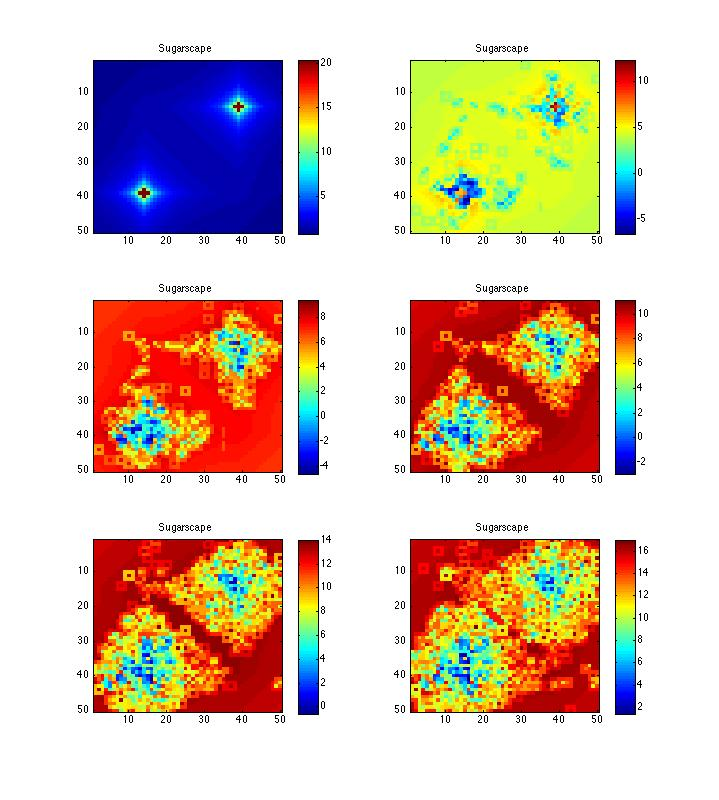
\includegraphics[scale=.30]{sugar.jpg}}
		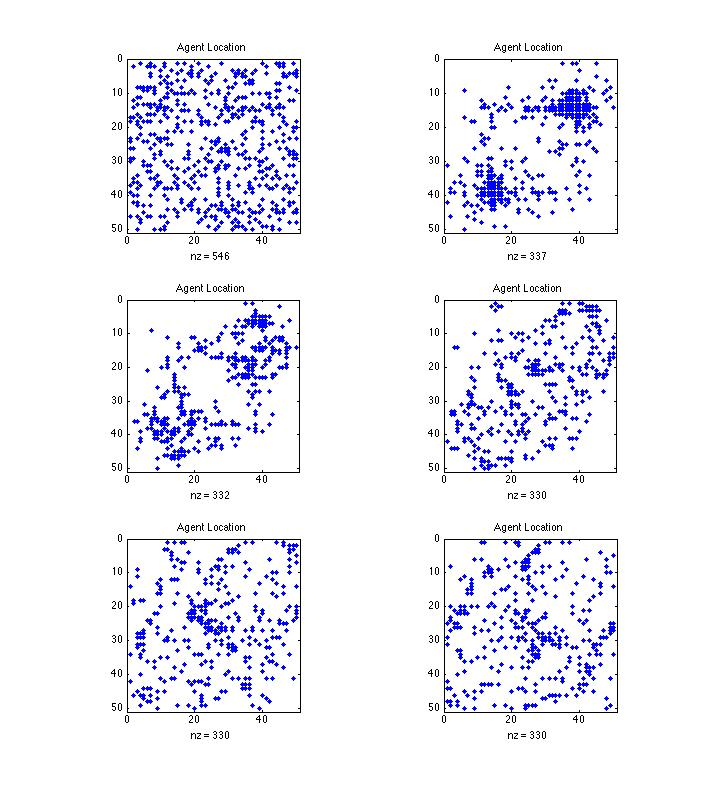
\includegraphics[scale=.30]{agents.jpg} 
		\caption{Fish and Fishermen Distribution}
	\end{center}
\end{figure} 

Initially, all agents cluster towards the sugar peaks. However, as the density of fishermen increases, the peaks quickly become dead zones with no fish. This causes the agents to move outwards from the clusters towards the areas where there is no competition and thus more fish. 

\subsection{Analogs and Interpretations}
As mentioned before, this move away from clusters can be seen as an analog to the distribution of energy in the universe over time. Originally, all energy (fish) was clustered into high-density, low-entropy regions. These regions quickly destabilized and caused them to move towards a low-density, high-entropy distribution. This fulfills the Second Law of Thermodynamics, which states that the entropy of the universe always increases. \*

The agent's reaction to the destruction of prime fisheries is also informative for policy decisions. In response to the depletion of fish reserves, the agents move in their own self-interest towards regions with more fish and isolated from other agents. This in turn allows for the fish stocks to replenish themselves while still sustaining the fishermen, as seen by the number of dead-zones decreasing over time. This implies that in the absence of regulation, the fishing industry can be self-correcting and organically create a system that sustains both themselves and the ecosystem.

\section{Moving Forward} 
In the future, the model can be improved by performing statistical analysis at each iteration, namely the size and number of clusters. This can be accomplished by a density-based scan algorithm, which identifies clusters based on the densities of areas relative to the whole. This would provide an accurate measure of dispersion of the fishermen and fish, giving a quantitative measure of what is visually apparent. \*
Additionally, I would also like to change the spatial landscape of the environment, adding certain regions that consistently create more fish, i.e. a reef structure or zone with a favorable current. This would more accurately represent the underwater ecosystem and provides more information as to how agents will spatially distribute themselves in the real world.

\newpage

\section{Appendix}

\begin{figure}[ht]
	\begin{center}
		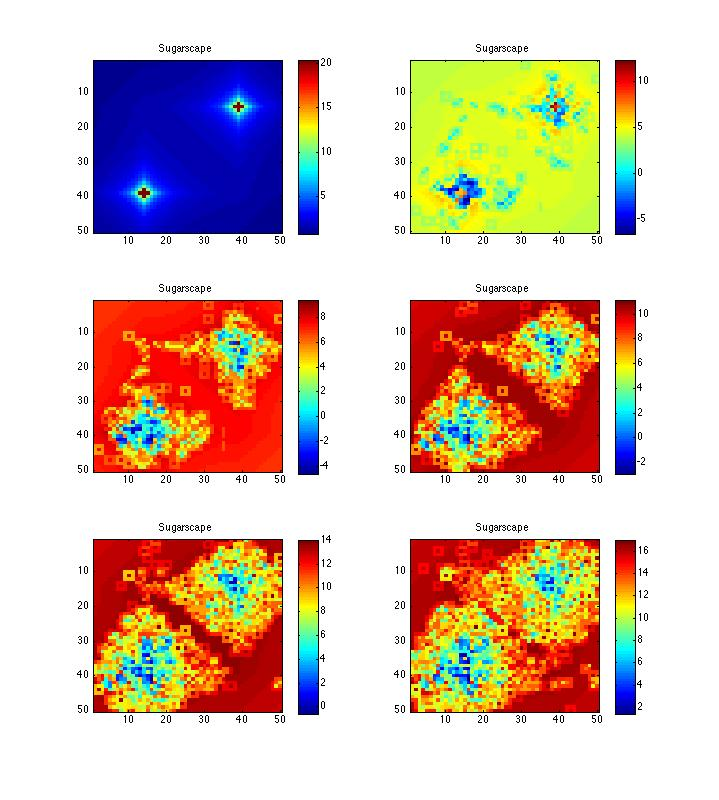
\includegraphics[scale=.75]{sugar.jpg}
		\caption{Fish Distribution}
	\end{center}
\end{figure} 

\begin{figure}[ht]
	\begin{center}
		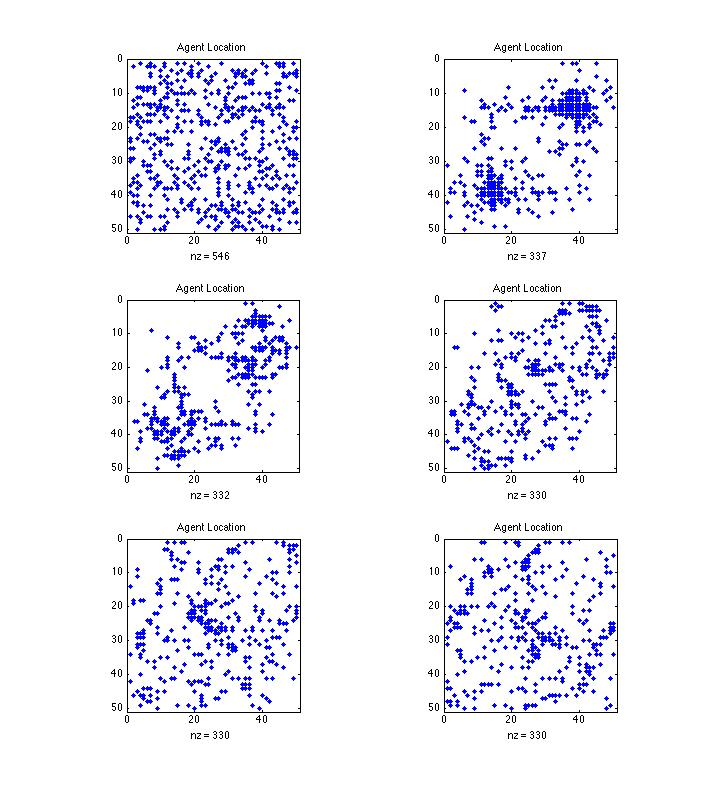
\includegraphics[scale=.75]{agents.jpg}
		\caption{Agent Distribution}
	\end{center}
\end{figure} 

\begin{figure}[ht]
	\begin{center}
		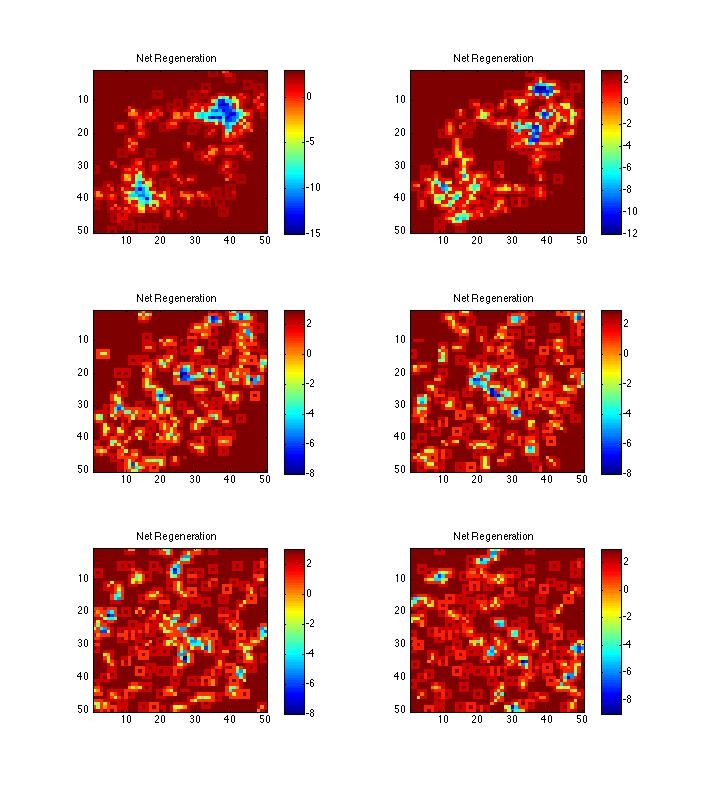
\includegraphics[scale=.75]{regen.jpg}
		\caption{Regeneration}
	\end{center}
\end{figure} 

\end{document}

